% chktex-file 2% chktex-file 29
% chktex-file 13
\documentclass{report}
\usepackage{setspace}
\usepackage[a4paper, total={7in, 9in}]{geometry}
\usepackage[fleqn]{amsmath}
\usepackage{empheq}
\usepackage{amssymb}
\usepackage{amsthm}
\usepackage{gensymb}
\usepackage[fleqn]{cases}
\usepackage{multicol}
\usepackage{color}
\usepackage{stix}
\usepackage{chngcntr}
\usepackage{tikz}
\usepackage{enumitem}
\usepackage{pgfplots}
\usetikzlibrary{calc,matrix,arrows}
\usetikzlibrary{decorations.pathmorphing,patterns}

\counterwithout{equation}{chapter}
\setlength{\columnseprule}{1pt}
\setlength{\columnsep}{24pt}
\setcounter{chapter}{14}
\hfuzz=100pt

\newcommand{\pgfplotsdrawaxis}{\pgfplots@draw@axis}
\makeatother
\pgfplotsset{only axis on top/.style={axis on top=false, after end axis/.code={
                    \pgfplotsset{axis line style=opaque, ticklabel style=opaque, tick style={thick,opaque},
                        grid=none}\pgfplotsdrawaxis}}}

\newtheorem{theorem}{Theorem}

\begin{document}
\newcommand{\sol}[1]{

    \noindent \textbf{Sol.}
}
\newcommand{\prooff}[1]{

    \noindent \textbf{Proof.}
}
\newcommand\m[1]{\begin{pmatrix}#1\end{pmatrix}}
\newcommand\vm[1]{\begin{vmatrix}#1\end{vmatrix}}
\newenvironment{amatrix}[1]{%
    \left(\begin{array}{@{}*{#1}{c}|c@{}}
        }{%
    \end{array}\right)
}
\begin{titlepage}
    \raggedleft{}
    \rule{1pt}{\textheight}
    \hspace{0.02\textwidth}
    \parbox[b]{0.75\textwidth}{

    {\Huge\bfseries Solution Book of \\[0.5\baselineskip] Mathematic}\\[2\baselineskip]
    {\large\textit{Ssnior 2 Part I}}\\[4\baselineskip]
    {\Large\textsc{MELVIN CHIA}}

    \vspace{0.5\textheight}

    {\noindent Written on 9 October 2022}\\[\baselineskip]
    }

\end{titlepage}

\doublespacing{}
\tableofcontents
\singlespacing{}
\newpage

\begin{multicols}{2}

    \section{Linear Inequalities of Two Variables}

    \subsection*{Solution of Linear Inequalities of Two Variables}

    A linear inequality of two variables is inequality with two variables involved.

    For any linear equation of two variables, there are infinitely many solutions.
    These solutions can be graphed in the appropriate half of a rectangular
    coordinate plane.

    \subsection{Practice 10}

    Express the solution of the following linear inequalities in graph form:

    \begin{enumerate}
        \item $x + 3y < 6$
              \sol{}
              \begin{center}
                  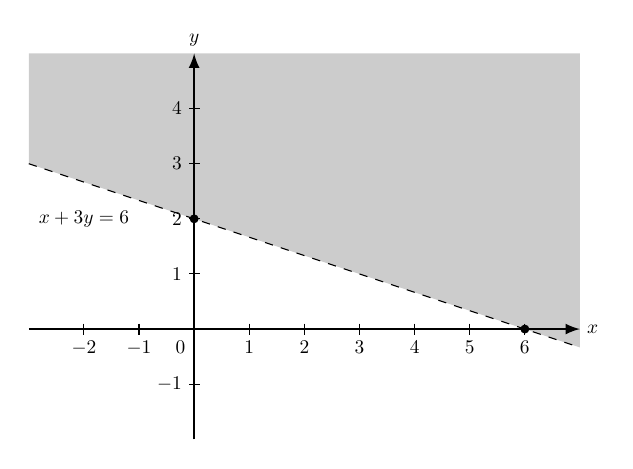
\begin{tikzpicture}[transform shape,scale=0.7]
                      \draw[draw=none,fill, color=black!20](-3,5)--(-3,3)--(7,-0.3333)--(7,5)--cycle;
                      \draw [-latex,thick](-3,0) -- (7,0) node[right] {$x$} coordinate(x axis);
                      \foreach \x in {-2,-1,1,2,3,4,5,6}
                      \draw (\x,0.1) -- (\x,-0.1) node [below] {$\x$};
                      \foreach \y in {-1,1,2,3,4}
                      \draw (0.1,\y) -- (-0.1,\y) node [left] {$\y$};
                      \draw [-latex,thick](0,-2) -- (0,5) node[above] {$y$} coordinate(y axis);
                      \node at (-0.25,-0.3375) {0};
                      \draw[color=black,dashed,domain=-3:7] plot (\x,-1/3*\x+2);
                      \node at (-2,2) {$x + 3y = 6$};
                      \filldraw[black] (0,2) circle (2pt);
                      \filldraw[black] (6,0) circle (2pt);
                  \end{tikzpicture}
              \end{center}

        \item $2x - 5y \leq 10$
              \sol{}
              \begin{center}
                  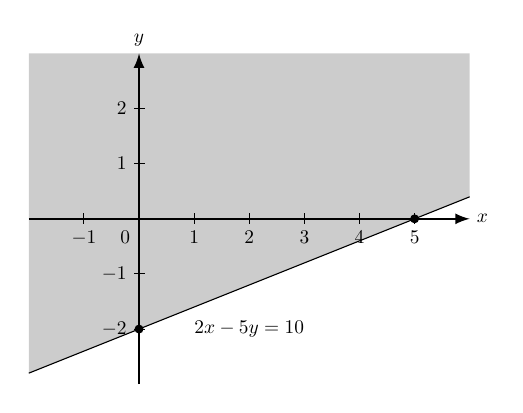
\begin{tikzpicture}[transform shape,scale=0.7]
                      \draw[draw=none,fill, color=black!20](-2,3)--(-2,-2.8)--(6,0.4)--(6,3)--cycle;
                      \draw [-latex,thick](-2,0) -- (6,0) node[right] {$x$} coordinate(x axis);
                      \foreach \x in {-1,1,2,3,4,5}
                      \draw (\x,0.1) -- (\x,-0.1) node [below] {$\x$};
                      \foreach \y in {-2,-1,1,2}
                      \draw (0.1,\y) -- (-0.1,\y) node [left] {$\y$};
                      \draw [-latex,thick](0,-3) -- (0,3) node[above] {$y$} coordinate(y axis);
                      \node at (-0.25,-0.3375) {0};
                      \draw[color=black,domain=-2:6] plot (\x,2/5*\x-2);
                      \node at (2, -2) {$2x - 5y = 10$};
                      \filldraw[black] (0,-2) circle (2pt);
                      \filldraw[black] (5,0) circle (2pt);
                  \end{tikzpicture}
              \end{center}

        \item $4y - x + 8 > 0$

        \item $3x + 2y \leq 9$
    \end{enumerate}

\end{multicols}
\end{document}